\documentclass[preprint,proceedings]{rmaa}

% These are some I use in typesetting example code
\newcommand{\bs}{\textbackslash}
\newcommand{\CS}[1]{\texttt{\textbackslash #1}}
% roman subscripts in math
\newcommand{\Sub}[1]{_\mathrm{#1}}
% a command to specify possible linebreak points in an email address 
\newcommand{\D}{\discretionary{}{}{}}

%%%
%%% Article preamble commands (title, authors, abstract, etc.) 
%%% None of these produce any output themselves, they just set things 
%%% up for \maketitle
%%%

% This is only used for making the header for the preprint version
\SetYear{2016}
\SetConfTitle{XV LARIM}

% Please use mixed case here, since this title gets propagated onto
% the web page, ADS entry, etc. 
\title{Influence of galaxy rotation and outflows on the Lyman Alpha spectral line}

\author{M. C. Remolina-Guti\'errez\altaffilmark{1}, J. E. Forero-Romero\altaffilmark{1} 
and J. N. Garavito-Camargo\altaffilmark{2}}

\altaffiltext{1}{Departamento de F\'isica, Universidad de los Andes, Cra 1 18A-10, Bloque Ip, Bogot\'{a}, Colombia.}
\altaffiltext{2}{Department of Astronomy, The University of Arizona, 933 North Cherry Ave Tucson, AZ 85721, Arizona, United States of America.}

% List of authors used to construct table of contents
\listofauthors{M. C. Remolina-Guti\'errez \& J. E. Forero-Romero \& J. N. Garavito-Camargo}
% Each author in Surname, Initials format, used in generating Author
% Index entries.
\indexauthor{Remolina-Guti\'errez, M. C.}
\indexauthor{Forero-Romero, J. E.}
\indexauthor{Garavito-Camargo, J. N.}


% No \abstract or \resumen for poster papers

% Keywords must be from the standard list and in alphabetical order. 
\addkeyword{galaxy simulations}
\addkeyword{lyman alpha emitters}
\addkeyword{radiative transfer}


%%%
%%% Beginning of document proper
%%%
\begin{document}
% Typeset article header
\maketitle 
%%%Resumen en Español%%%
\boldabstract{
  En esta presentaci\'on mostramos la influencia que tienen la rotaci\'on y los outflows
  de las galaxias Lyman Alpha Emitters (LAEs) en su espectro. Creamos un nuevo modelo de LAE
  que consiste en una distribuci\'on esferica y homogenea de \'atomos de Hidr\'ogeno que gira como cuerpo
  solido y que se expande radialmente debido a outflows. Por medio de simulaciones de transferencia
  radiativa y en base a la din\'amica de movimiento, generamos la l\'inea de emisi\'on Lyman Alpha (Ly$\alpha$)
  resultante. Finalmente analizamos la morfología de \'esta l\'inea y las implicaciones que podría tener en
  la estimación de parámetros físicos de las LAEs. 
}

%%%Abstract%%%

\boldabstract{
  In this talk we show the influence of rotation and outflows of Lyman Alpha Emitters (LAEs)
  galaxies in their spectrum. We create a new model of LAE that consists of a spherical homogeneus distribution 
  of Hydrogen atoms undergoing a solid body rotation and a radial expansion due to outflows. We generate
  the galaxy's Lyman Alpha (Ly$\alpha$) emission line using radiative transfer simulations based on its 
  motion dynamics. Finally, we analyze the morpholgy of the line and the implications it might have on the
  estimations of LAEs' physical parameters.
}

Galaxies detected through their distinctive Ly$\alpha$ emission are known as Lyman Alpha 
Emitters (LAEs). Typical LAEs are star-forming and have a low dust content. Additional
dynamical characteristics of a LAEs' insterstellar medium can be derived by studying its
Ly$\alpha$ line morphology and comparing it against theoretical models.

{\bf A new LAE model}.
In this work we create a new LAE model that considers the galaxy as a spherical distribution
of Hydrogen atoms. It combines the effect of bulk rotation and outflows in the form of solid body
rotation and radial expansion. So our model can be parametrized by 4 variables: rotation velocity
$v_{\mathrm{rot}}$, outflow velocity $v_{\mathrm{out}}$, optical depth $\tau$ and viewing angle
$\theta$. Where $\tau$ represents the number of H atoms in the galaxy and $\theta$ represents the
angle at which the observer can detect the photons that escaped the galaxy.

{\bf Simulation}.
We include these dynamical effects into a modified version of a Monte Carlo radiative transfer code
called CLARA. This in order to study the parameters' impact into the the Ly$\alpha$ line morphology.

\begin{figure}[h!]
	\centering
	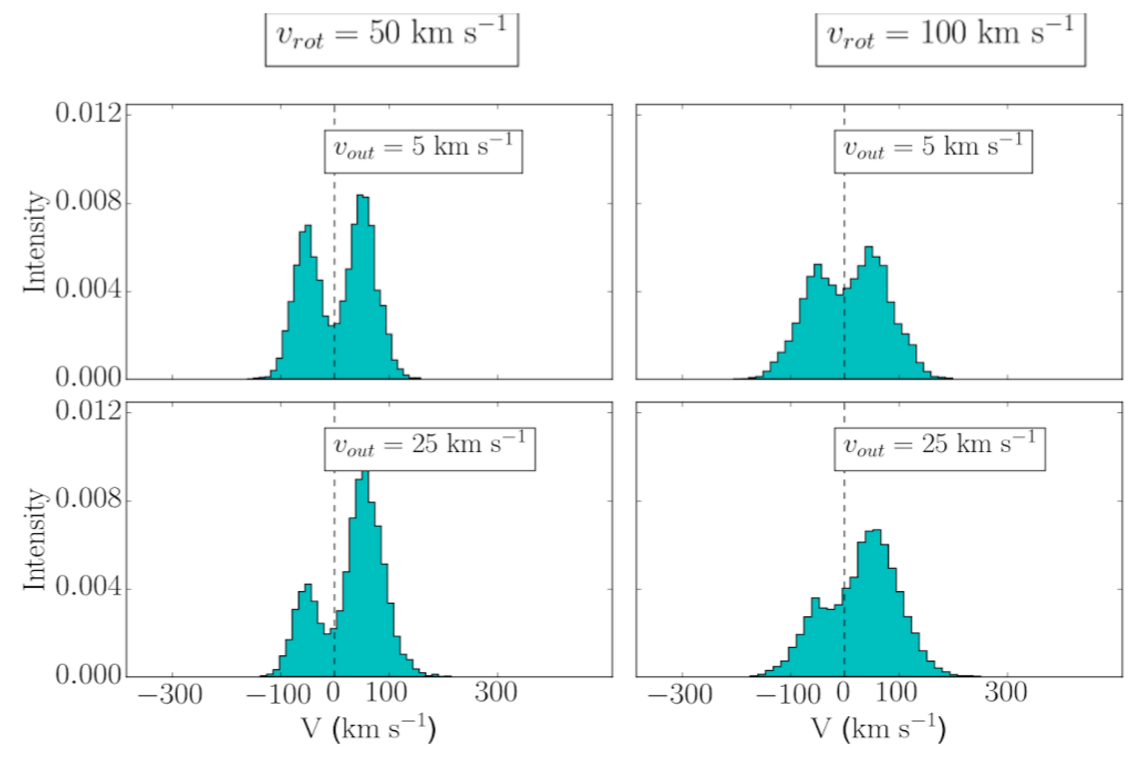
\includegraphics[width=0.45\textwidth]{spectra}
	\label{fig1}
	\caption{Resulting simulated spectra for $\tau=10^5$ and $\theta=90^\circ$.}
\end{figure}

{\bf Results}. We find that rotation alone does have an impact on the Ly$\alpha$ morphology. 
However, together with the outflows, the new model can reproduce double peak asymmetry in the line 
and can induce a Doppler shift shift in the rotation only spectrum. We are able to reproduce LAEs' main
observed features with physically motivated parameters for the rotational and outflow velocities.
We present fits of this model to some observational spectra to argue that both rotation and outflows
have to be taken into account for a proper estimation of a LAE's physical parameters. 


\begin{thebibliography}

\bibitem{1} J. E. {Forero-Romero}, G. {Yepes}, S. {Gottl{\"o}ber}, S. R. {Knollmann},
			A. J. {Cuesta}, F. {Prada}.
  			{CLARA's view on the escape fraction of Lyman {$\alpha$} photons in high-redshift galaxies},
  			MNRAS, 415, August 2011.
\bibitem{2} J. N. {Garavito-Camargo}, J. E. {Forero-Romero}, M. {Dijkstra}.
			{The Impact of Gas Bulk Rotation on the Ly{$\alpha$} Line},
			ApJ, 795, November 2014.

\end{thebibliography} 

\end{document}
